
\section{Preliminary  Comparisons}
\label{Sec:Comparison}

\subsection{Measuring error}

\begin{frame}
  \frametitle{Measuring errors}
  \begin{block}{Full error criteria}
    \begin{equation}
      \label{eq:error-1}
      \mbox{error} = \frac{\|F^\nat_\vitwo(r)\|}{\|q\|}.
    \end{equation}
  \end{block}
  \begin{block}{Cheap error}
    \begin{equation}
      \label{eq:error-2}
      \mbox{error}_{\mbox{cheap}} = \frac{\|r_{k+1}-r_{k}\|}{\|r_k\|}.
    \end{equation}
    The tolerance of solver is then self-adapted in the loop to meet the required tolerance based on the error given by~\eqref{eq:error-1}.
  \end{block}
\end{frame}

\subsection{Performance profiles}
\frame{
  \frametitle{Performance profiles~\cite{Dolan.More2002}}

  \begin{itemize}
  \item Given a set of problems $\mathcal P$
  \item Given a set of solvers $\mathcal S$  
  \item A performance measure for each problem  with a solver $t_{p,s}$ (cpu time, flops, ...)
  \item Compute the performance ratio
    \begin{equation}
      \label{eq:perf-ratio}
      \tau_{p,s} =    \Frac{t_{p,s}}{\min_{s\in\mathcal S} t_{p,s}} \geq 1
    \end{equation}
  \item Compute the performance profile $\rho_s(\tau) : [1,+\infty]\rightarrow [0,1]$ for each solver $s\in \mathcal S$
    
    \begin{equation}
      \rho_s(\tau) = \Frac{1}{|\mathcal P|}\big|\{p\in \mathcal P\mid \tau_{p,s} \leq \tau    \}\big|\label{eq:perf}
  \end{equation}
  The value of $\rho_s(1)$ is the probability that the solver $s$ will win over the rest of the solvers.
  \end{itemize}
  
  
}
\def\ssep{1.5mm}

\frame{
  
\def\figillus{0.15\textheight}
\begin{figure}
  \centering
  \subfloat[Cubes\_H8]{\includegraphics[height=\figillus]{figure/Cubes_H8_5.png}$\quad$}
  \subfloat[LowWall\_FEM]{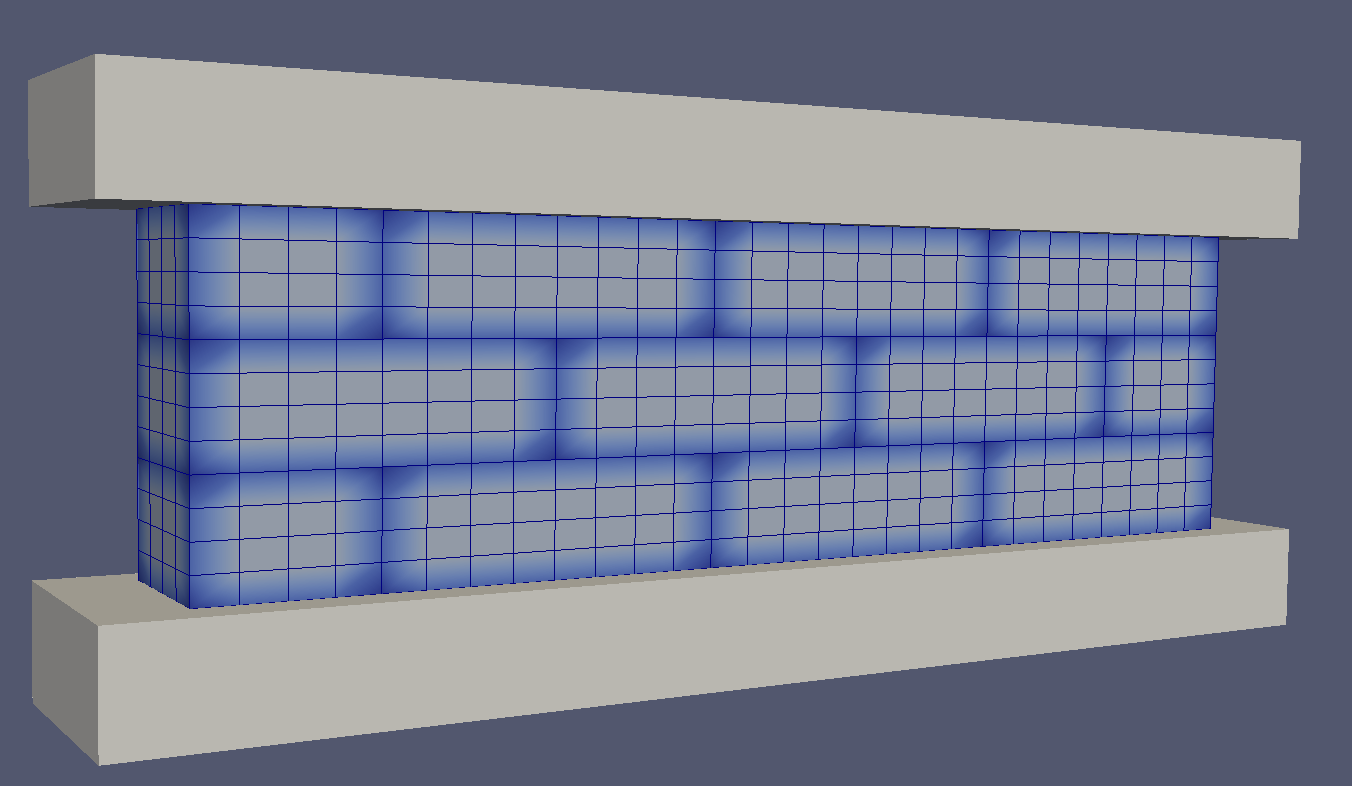
\includegraphics[height=\figillus]{figure/LowWall_FEM.png}}
  \subfloat[Aqueduct\_PR]{\includegraphics[height=\figillus]{figure/Aqueduc_PR.png}$\quad$}
  \subfloat[Bridge\_PR]{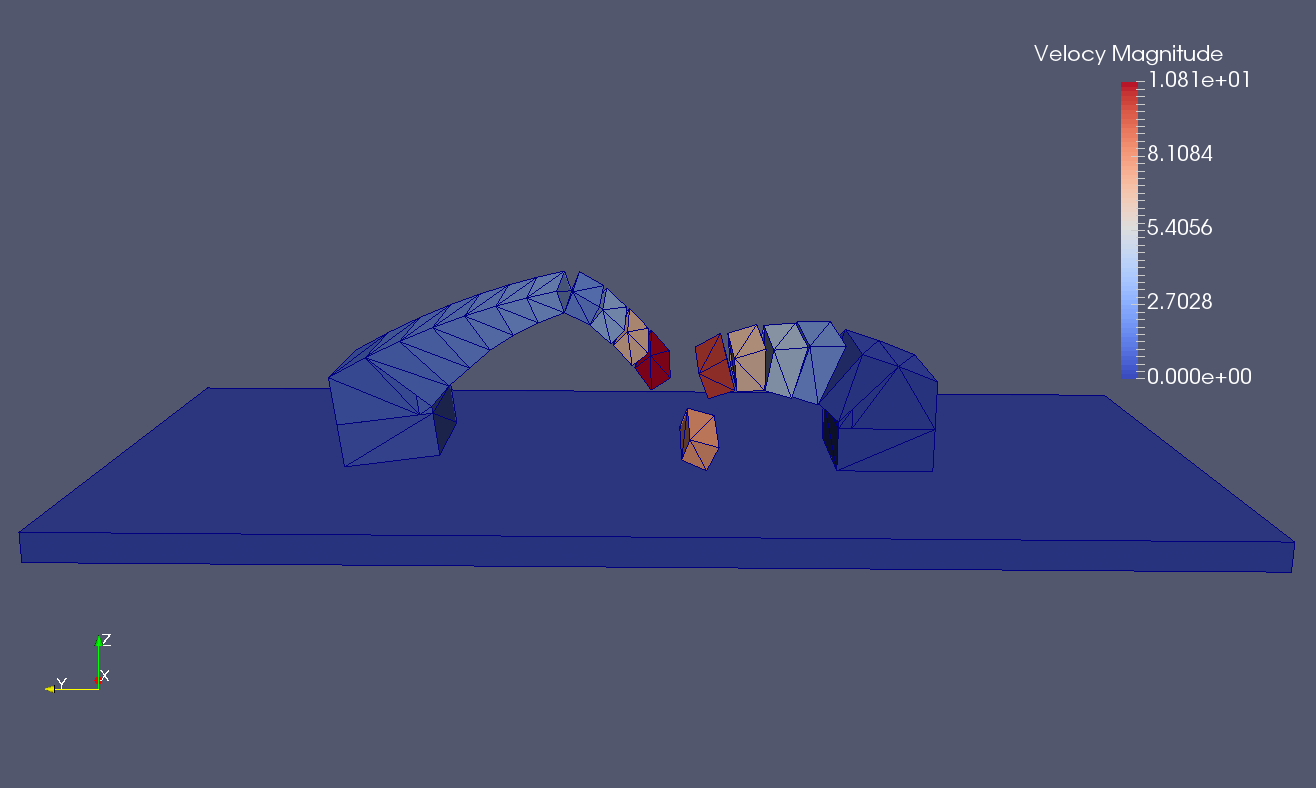
\includegraphics[height=\figillus]{figure/Bridge_PR_1.png}}\\
  \subfloat[100\_PR\_Periobox]{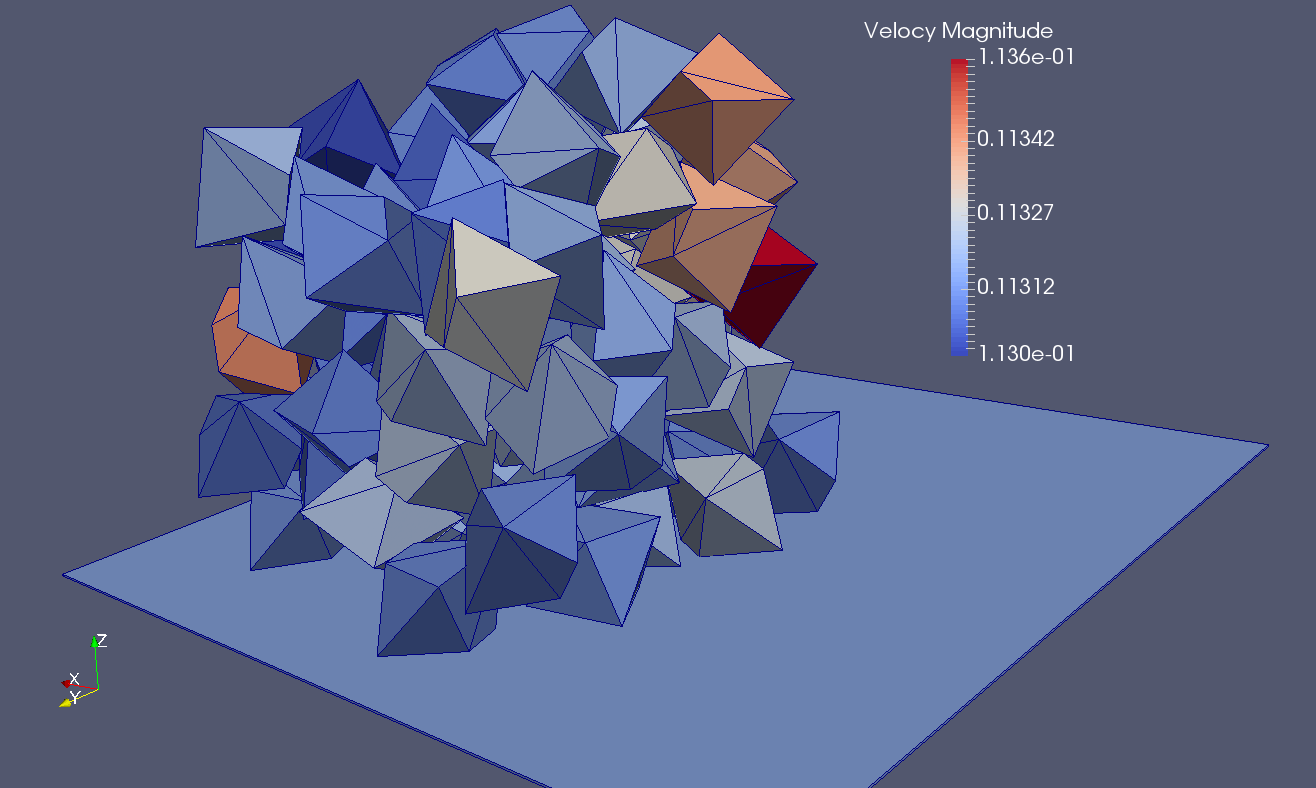
\includegraphics[height=\figillus]{figure/100_PR_PerioBox.png}$\quad$}
  \subfloat[945\_SP\_Box\_PL]{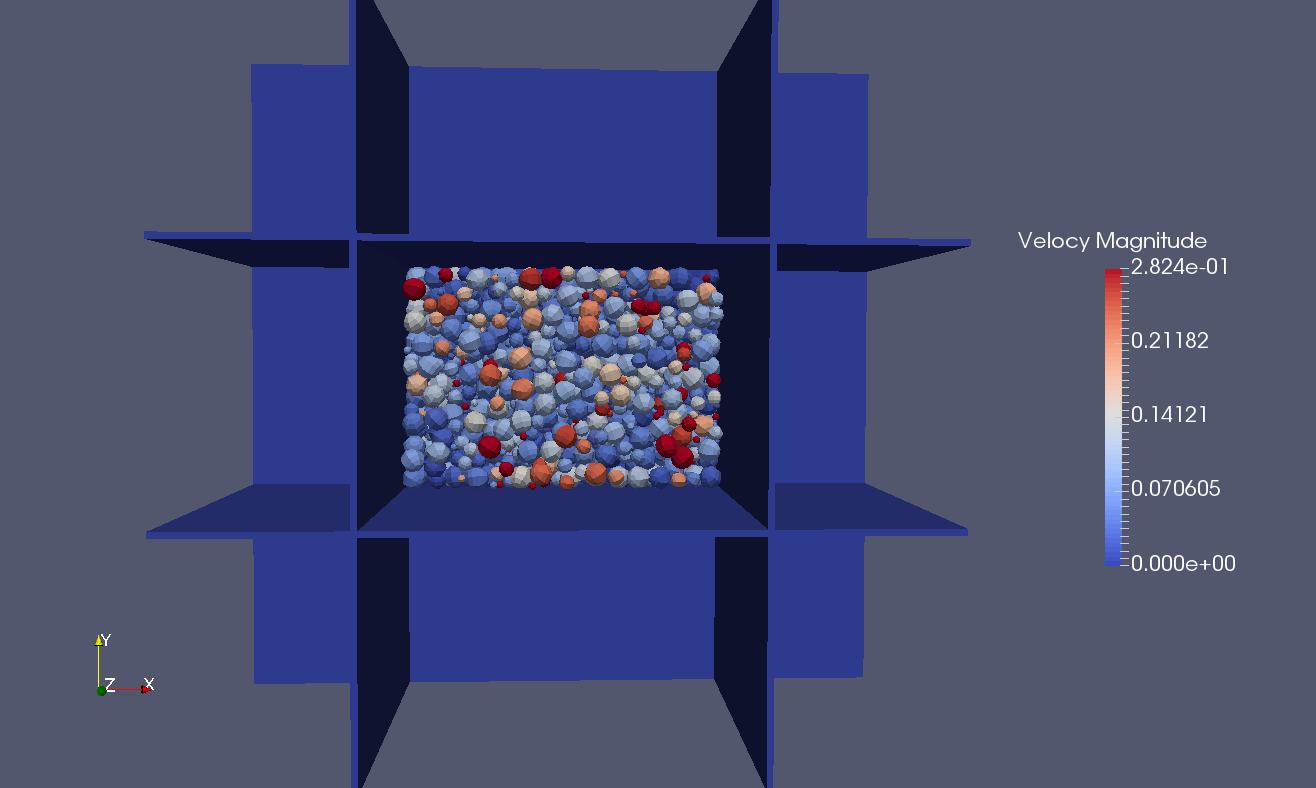
\includegraphics[height=\figillus]{figure/945_SP_Box_PL.png}}
  \subfloat[Capsules]{\includegraphics[height=\figillus]{figure/Capsules.png}$\quad$}
  \subfloat[Chain]{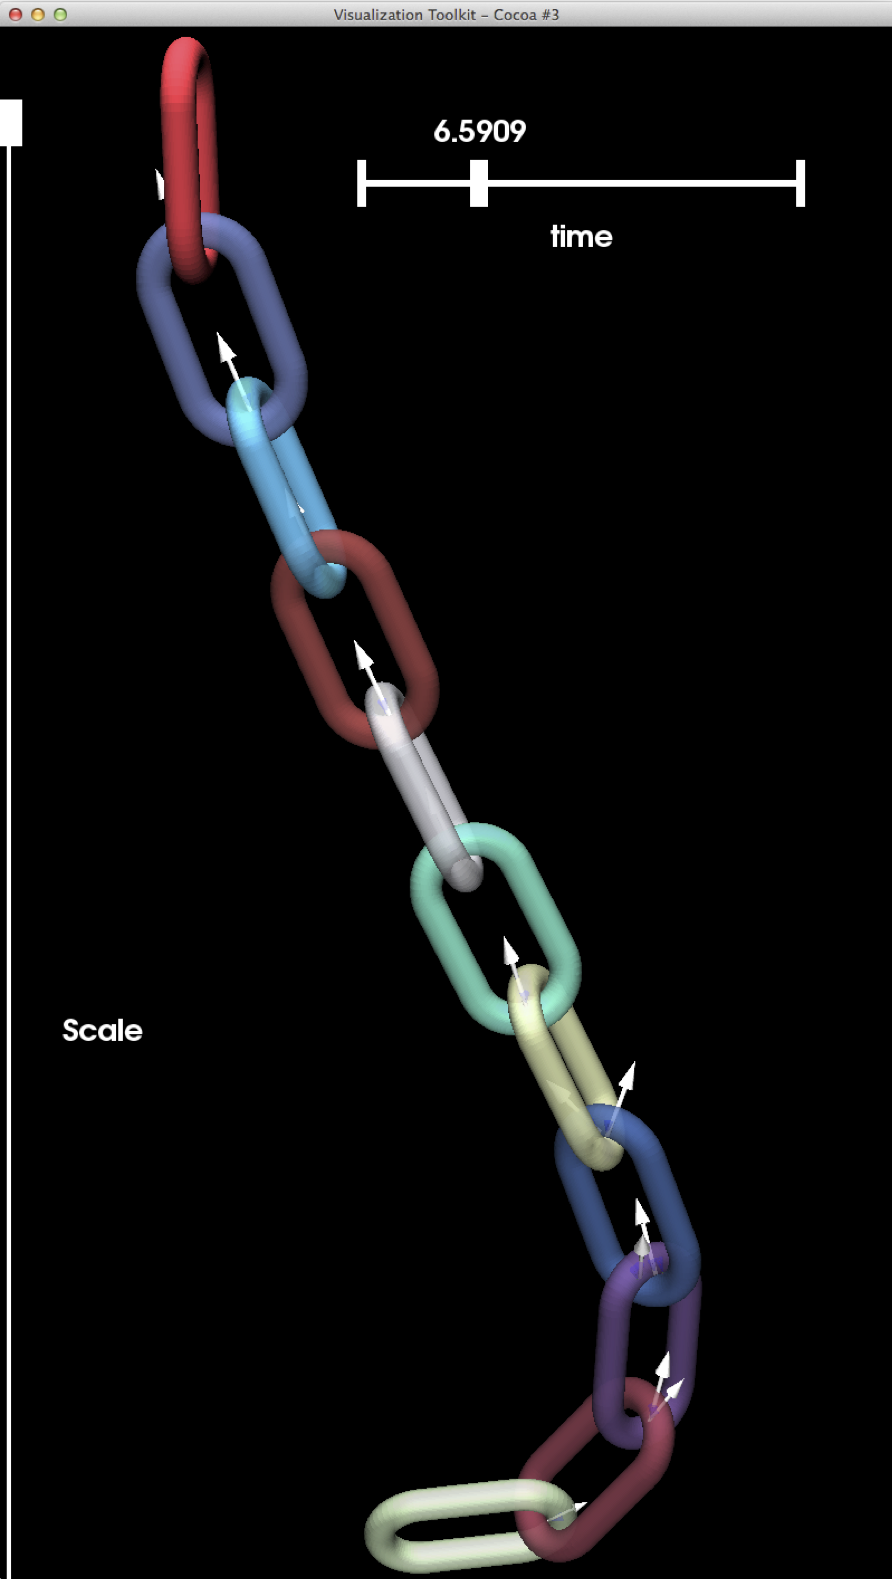
\includegraphics[height=\figillus]{figure/Chains.png}$\quad$}\\
  \subfloat[KaplasTower]{\includegraphics[height=\figillus]{figure/KaplasTower.png}$\quad$}
  \subfloat[BoxesStack]{$\quad$$\quad$\includegraphics[height=\figillus]{figure/BoxesStack.png}$\quad$$\quad$}
  \subfloat[Chute\_1000, Chute\_4000, Chute\_local\_problems]{$\quad$$\quad$$\quad$$\quad$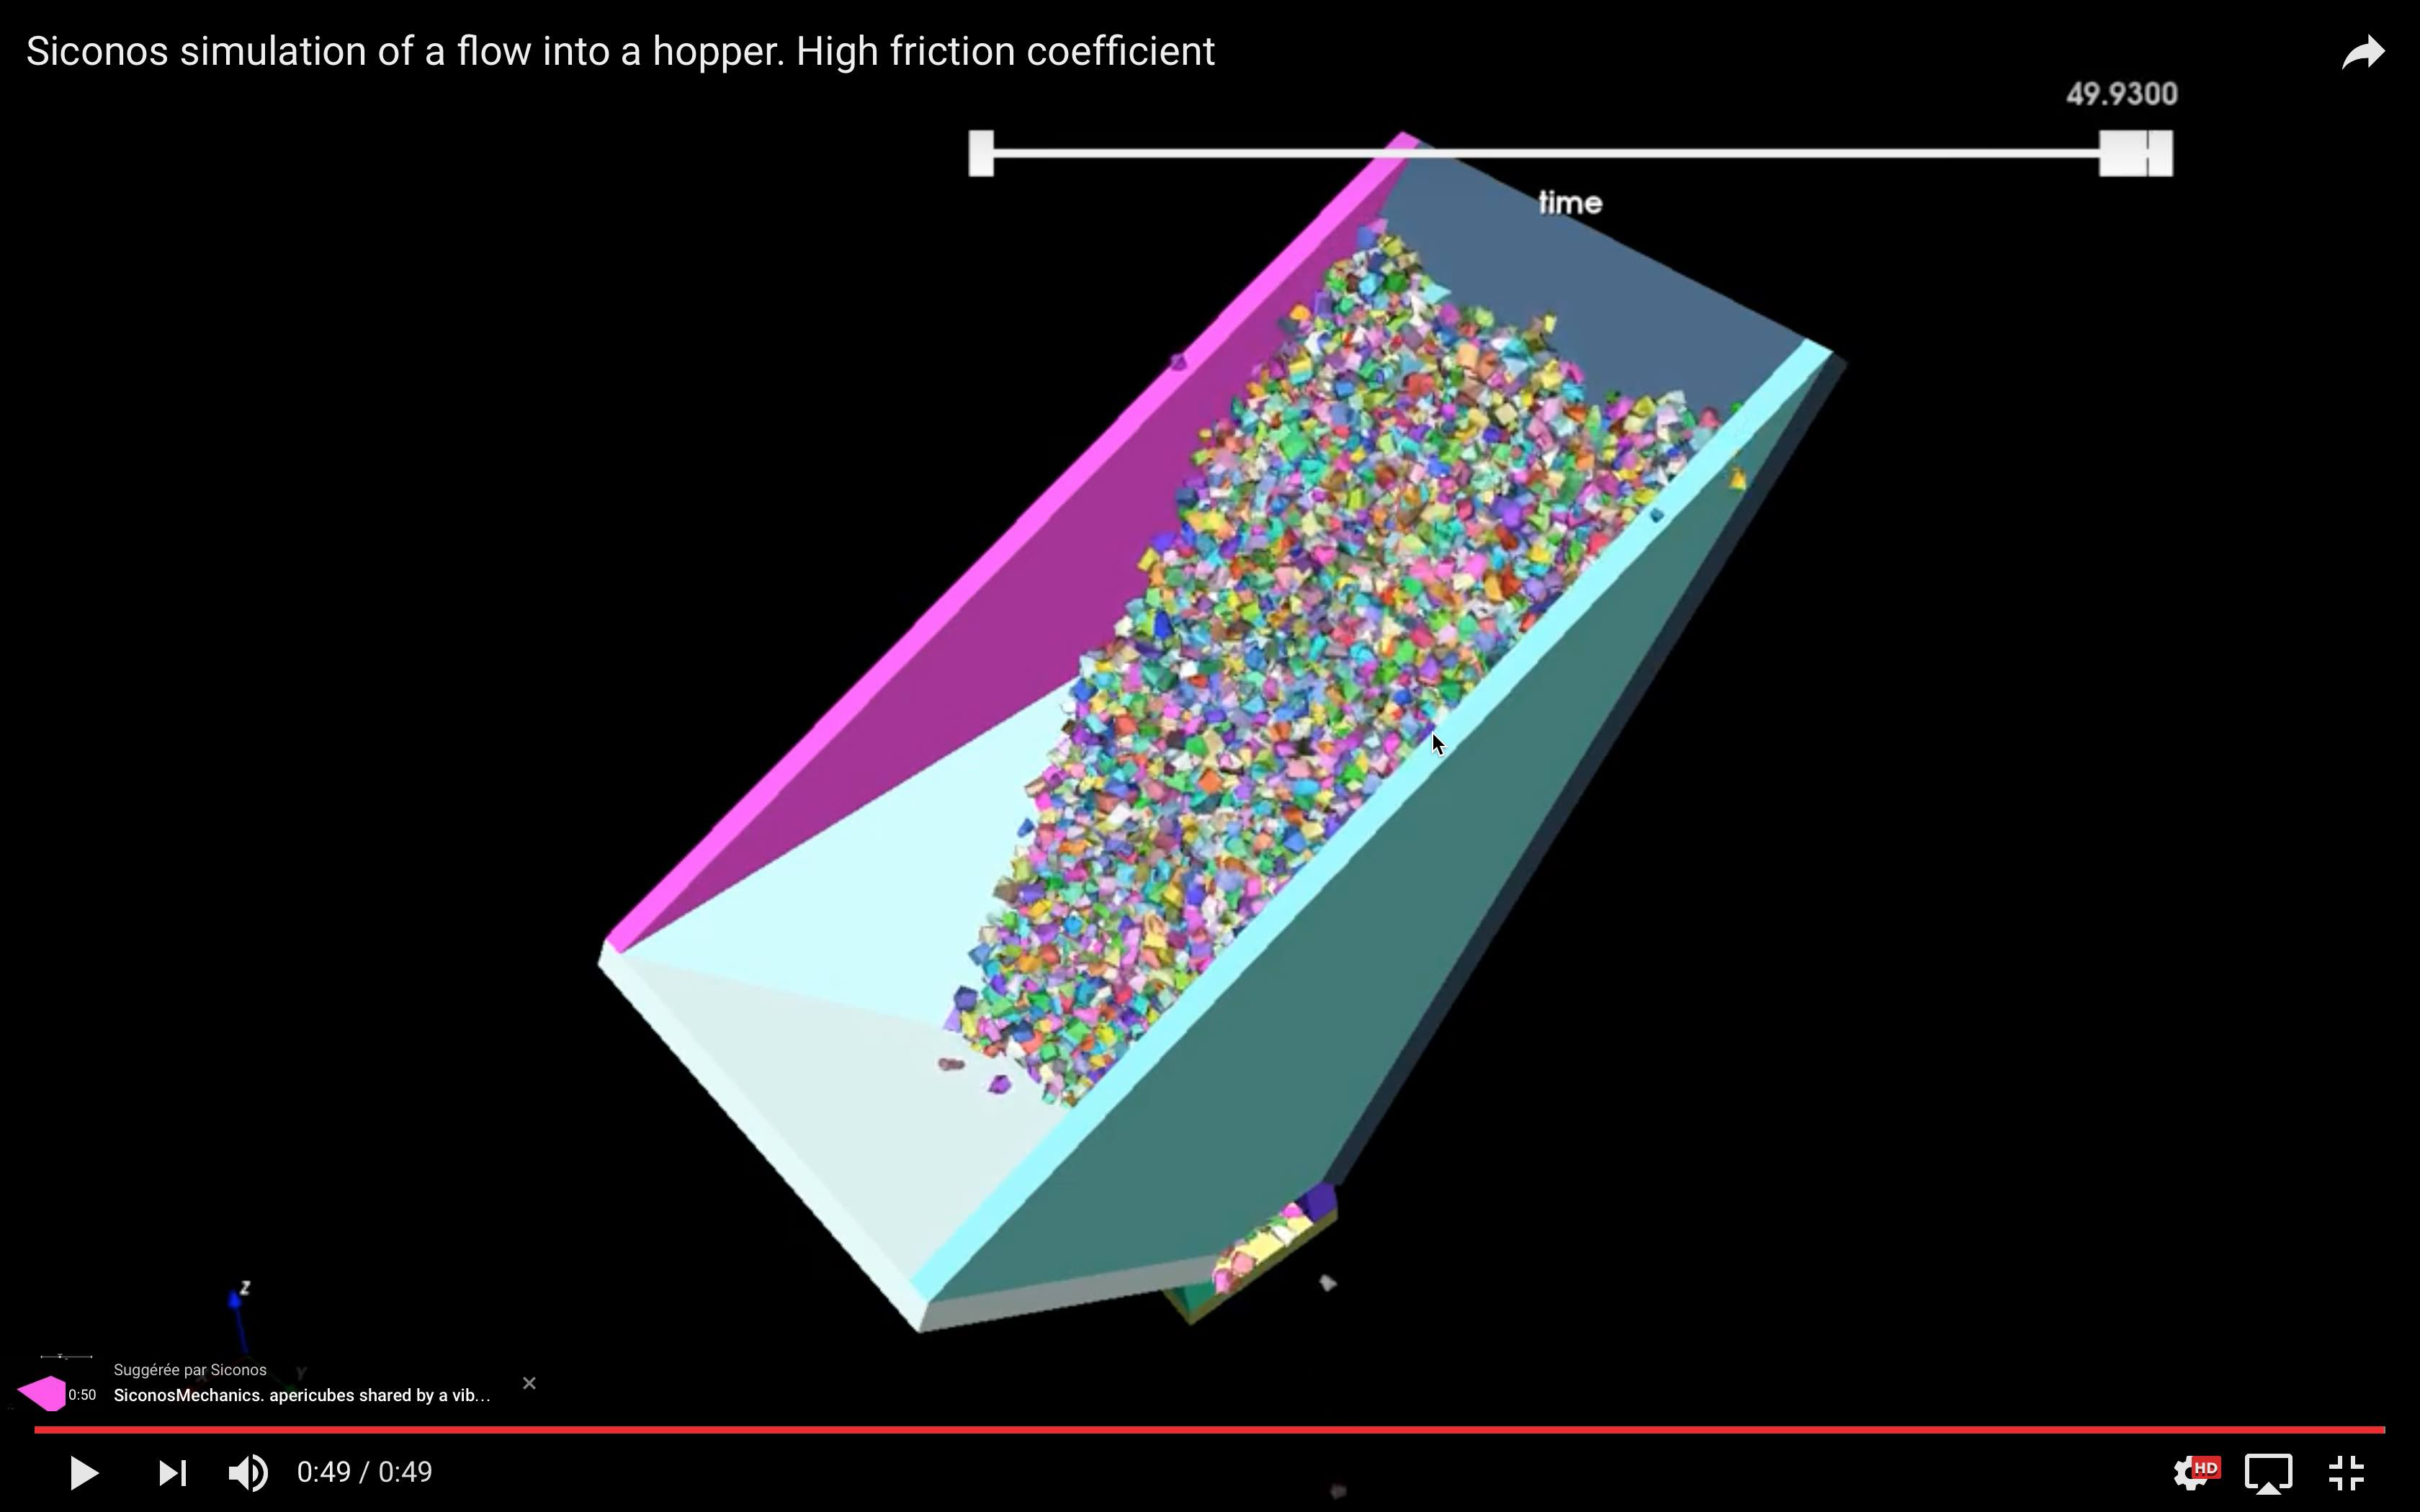
\includegraphics[height=\figillus]{figure/Chute_1000_light.jpg}$\quad$$\quad$$\quad$$\quad$}
  \caption{Illustrations of the FClib test problems}
  \label{fig:fclib}
\end{figure}
}

\begin{frame}
  \scriptsize
  \begin{table}
  \newcolumntype{H}{>{\setbox0=\hbox\bgroup}c<{\egroup}@{}} \begin{tabular}{|l|l|l|l|l|l|l|l|H@{\hspace*{-\tabcolsep}}|H@{\hspace*{-\tabcolsep}}|H@{\hspace*{-\tabcolsep}}|}
  \hline
  Test set
  & code
  & \parbox[t]{2mm}{\rotatebox[origin=c]{-90}{  friction coefficient $\mu$  }}
  & \parbox[t]{2mm}{\rotatebox[origin=c]{-90}{ \# of problems }}
  & \parbox[t]{2mm}{\rotatebox[origin=c]{-90}{ \# of d.o.f. }}
  & \parbox[t]{2mm}{\rotatebox[origin=c]{-90}{ \# of contacts }}
  & \parbox[t]{2mm}{\rotatebox[origin=c]{-90}{contact density $c$}}
  %& \parbox[t]{2mm}{\rotatebox[origin=c]{-90}{rank(W)}}
  & \parbox[t]{2mm}{\rotatebox[origin=c]{-90}{rank ratio(W)}}
  & \parbox[t]{2mm}{\rotatebox[origin=c]{-90}{cond(W)}}
  & \parbox[t]{2mm}{\rotatebox[origin=c]{-90}{cond(W) LSMR}}
  & \parbox[t]{2mm}{\rotatebox[origin=c]{-90}{$\mu(\|W-W^T\|)$}}
    \parbox[t]{2mm}{\rotatebox[origin=c]{-90}{symmetry of $W$}}
  \\
  \hline
  \hline
  Cubes\_H8\_2
  & LMGC90
  & 0.3
  & 15
  & 162
  & $[3:5]$
  & $[0.02:0.09]$
%  & $[6:15]$
  & 1
  & $[2.2.10^{1}:1.3.10^{3}]$
  & $[8.1.10^{5}:1.5.10^{6}]$
  & $3.2.10^{-4}$\\
   \hline
  Cubes\_H8\_5
  & LMGC90
  & 0.3
  & 50
  & 1296
  & $[17:36]$
  & $[0.02:0.09]$
%  & $[48:108]$
  & 1
  & $[3.3.10^{4}: 7.2.10^{4} ]$
  & $[1.3.10^{6}: 3.1.10^{6} ]$
  & $4.2.10^{-4}$\\
   \hline
  Cubes\_H8\_20
  & LMGC90
  & 0.3
  & 50
  & 55566
  & $[361:388]$
  & $[0.019:0.021]$
%  & $[1083:1164]$
  & 1
  & $[2.4.10^{5}: 2.5.10^{5} ]$
  & $[1.3.10^{6}: 5.2.10^{6} ]$
  &  $5.2.10^{-5}$\\
  \hline
  LowWall\_FEM
   & LMGC90
  & 0.83
  & 50
  & \{7212\}
  & $[624:688]$
  & $[0.28:0.29]$
%  & $[1873:2064]$
  & 1
  & --
  & $[9.3.10^{2}:5.0.10^{5}]$
  &  $5.2.10^{-2}$\\
  \hline
  Aqueduct\_PR
  & LMGC90
  & 0.8
  & 10
  & \{1932\}
  & $[4337:4811]$
  & $[6.81:7.47]$
%  & $[1934]$$
  & $[6.80:7.46]$
  & $[4.7.10^{7}:3.4.10^{8}]$
  & $[6.7.10^{1}:1.5.10^{2}]$
  &  $1.1.10^{-15}$\\
  \hline
  Bridge\_PR
  & LMGC90
  & 0.9
  & 50
  & \{138\}
  & $[70:108]$
  & $[1.5:2.3]$
%  & $[87:132]$
  & $[2.27:2.45]$
  & $[8.3.10^{4}:1.1.10^{5}]$
  & $[1.9.10^{3}:2.6.10^{4}]$
  & $5.8.10^{-18}$\\
  \hline
  100\_PR\_Periobox
  & LMGC90
  & 0.8
  & 106
  & \{606\}
  & $[14:578]$
  & $[0.2:3]$
%  & $[23:600]$
  & $[1.76:3.215]$
  & $[4.3.10^{2}:1.0.10^{6}]$
  & $[6.3.10^{5}:3.5.10^{6}]$
  & $8.8.10^{-20}$\\
  \hline
  945\_SP\_Box\_PL
  & LMGC90
  & 0.8
  & 60
  & \{5700\}
  & $[2322:5037]$
  & $[1.22:2.65]$
%  & $[5333:7617]$
  & $[1.0:2.66]$
  & $[2.2.10^{4}:4.4.10^{5}]$
  & $[2.9.10^{1}:9.2.10^{2}]$
  & $1.3.10^{-10}$\\
  \hline
  Capsules
  & Siconos
  & 0.7
  & 249
  & [96:600]
  & $[17:304]$
  & $[0.53:1.52]$
%  & $[47:587]$
  & $[1.08:1.55]$
  & --
  & $[4.8:1.6.10^{2}]$
  & $3.3.10^{-02}$\\
  \hline
  Chain
  & Siconos
  & 0.3
  & 242
  & \{60\}
  & $[8:28]$
  & $[0.5:1.3]$
%  & 53
  & $[1.05:1.6]$
  & $[7.4.10^{4}:4.0.10^{9}]$
  & $[1.5.10^{1}:4.7.10^{5}]$
  & $3.7.10^{-02}$\\
  \hline
  KaplasTower
  & Siconos
  & 0.7
  & 201
  & $[72:792]$
  & $[48:933]$
  & $[3.0:3.6]$
%  & $[72:792]$
  & $[2.0:3.53]$
  & $[67:2174]$
  & $[8:67]$
  & $5.4.10^{-08}$\\
  \hline
  BoxesStack
  & Siconos
  & 0.7
  & 255
  & $[6:300]$
  & $[1:200]$
  & $[1.86:2.00]$
%  & $[54:300]$
  & $[1.875:2.0]$
  & $[3.8.10^{4}:2.5.10^{7}]$
  & $[9.0:5.4.10^{3}]$
  & $2.23.10^{-14}$\\
  \hline
  Chute\_1000
  & Siconos
  & 1.0
  & 156
  & $[276:5508]$
  & $[74:5056]$
  & $[0.69:2.95]$
%  & $[222:8133]$
  & $[1.0:2.95]$
  & $[2.1.10^{1}:1.9.10^{3}]$
  & $6.6.10^{-02}$ \\
  \hline
  Chute\_4000
  & Siconos
  & 1.0
  & 40
  & $[17280:20034]$
  & $[15965:19795]$
  & $[2.51:3.06]$
  & --
  % & $[222:8133]$
  & --
  & $[5.5.10^{1}:9.0.10^{3}]$
  & $8.9.10^{-14}$\\
  \hline
  Chute\_local\_problems
  & Siconos
  & 1.0
  & 834
  & 3
  & 1
  & 1
%  & 3
  & 1
  & $[1.04:4.66]$
  & $[2.6:2.6.10^{1}]$
  & $1.76.10^{-09}$\\
  \hline
\end{tabular}
\caption{Description of the test sets of FCLib library (v1.0)}
\label{Tab:fclib}
\end{table}
\end{frame}


% \subsection{Chain}
% \frame{
%   \frametitle{First comparisons. Chain}
%   \begin{block}
%     {Hanging chain with initial velocity at the tip}
%     code: Siconos
%     $$ $$
%     \begin{minipage}{0.39\linewidth}
%       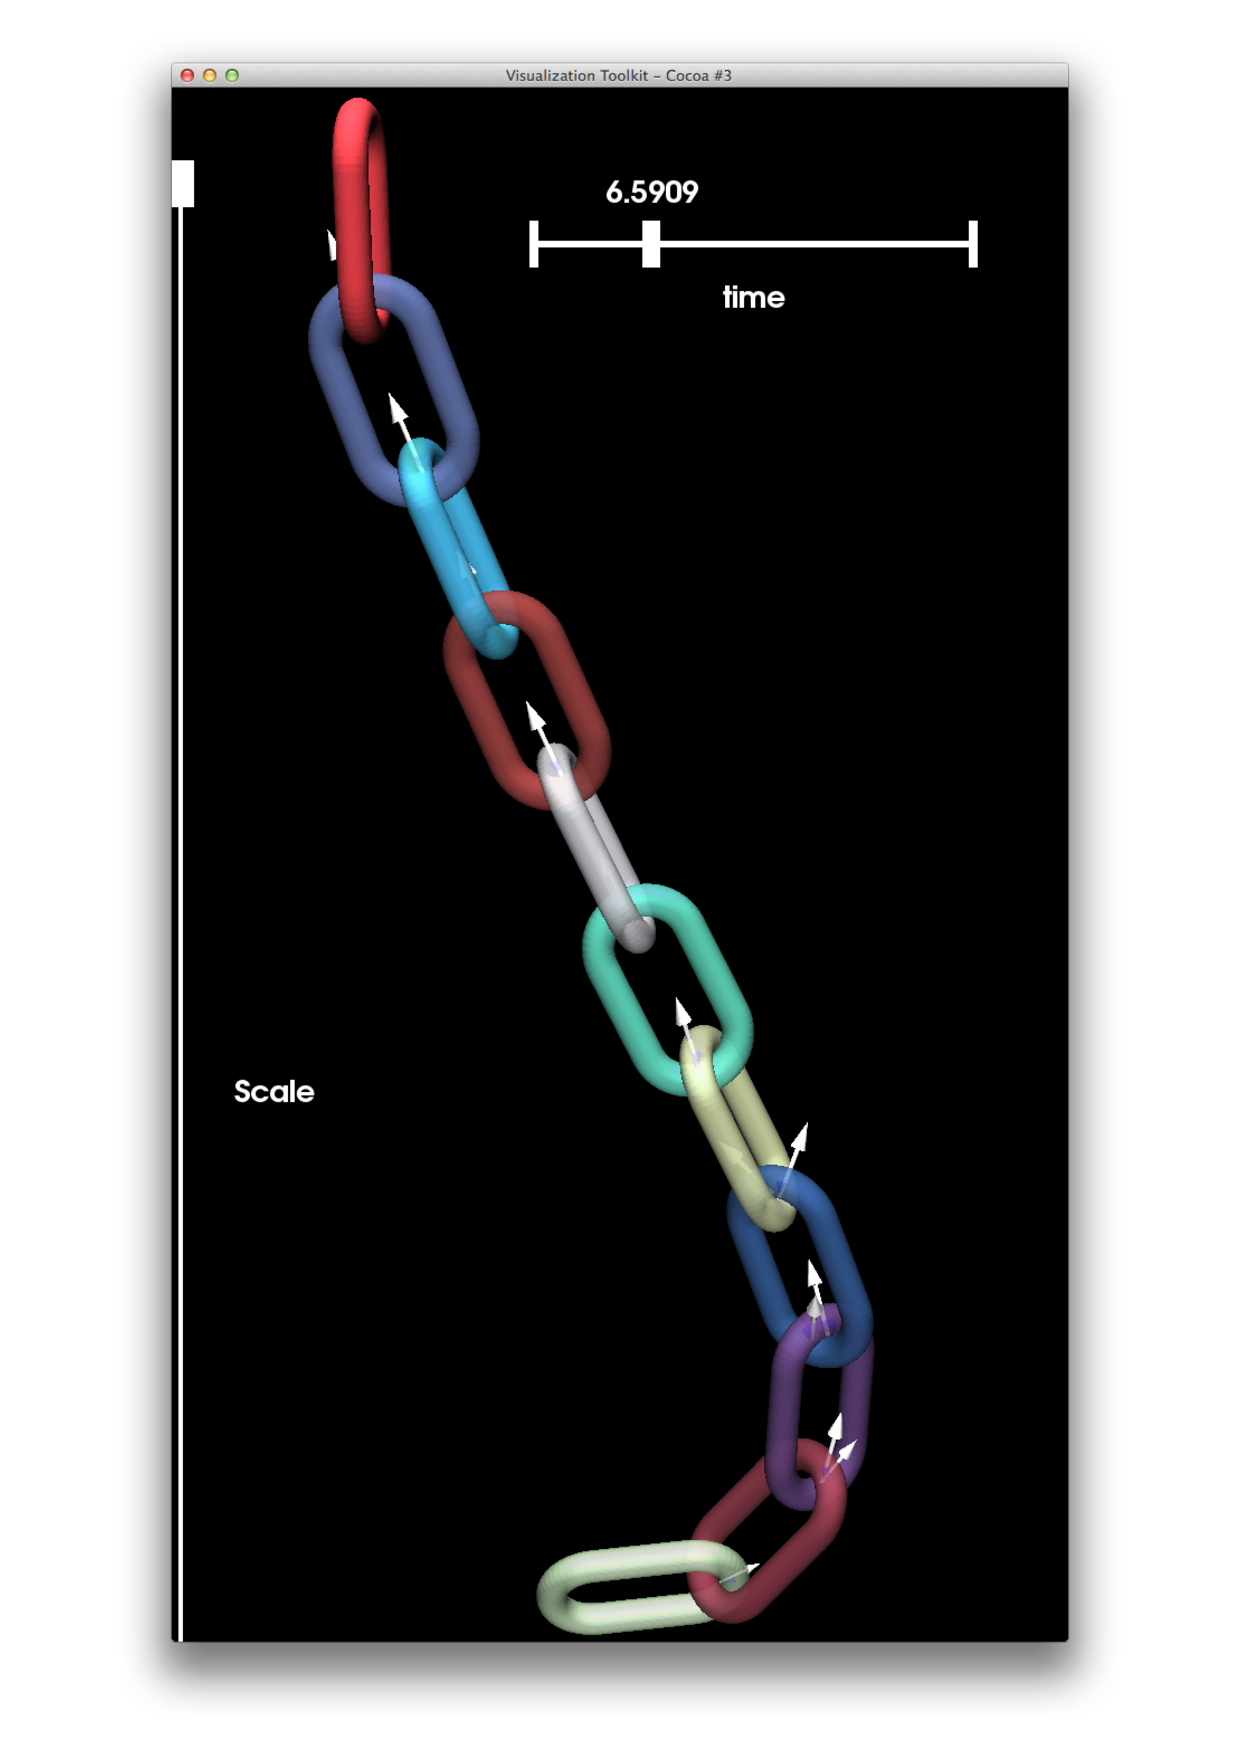
\includegraphics[width=1.0\textwidth]{Chains}
%     \end{minipage}
%     \begin{minipage}{0.49\linewidth}
%       \begin{tabular}{|p{0.7\textwidth}|c|}
%         coefficient of friction & $0.3$ \\[\ssep]
%         number of problems & 1514 \\[\ssep]
%         number of degrees of freedom & [48 : 60] \\[\ssep]
%         number of contacts & [8 :28] \\[\ssep]
%         required accuracy   & $10^{-8}$    
%       \end{tabular}
%     \end{minipage}
%   \end{block}

% }
% \frame{
%   \frametitle{First comparisons. Chain}
%   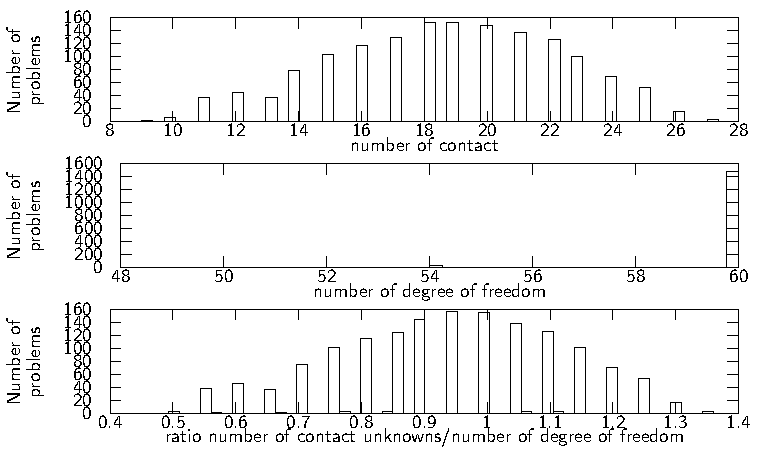
\includegraphics[width=1.10\textwidth]{distrib-Chain.pdf}
% }
% \frame{
%   \frametitle{First comparisons. Chain}
%     \centerline{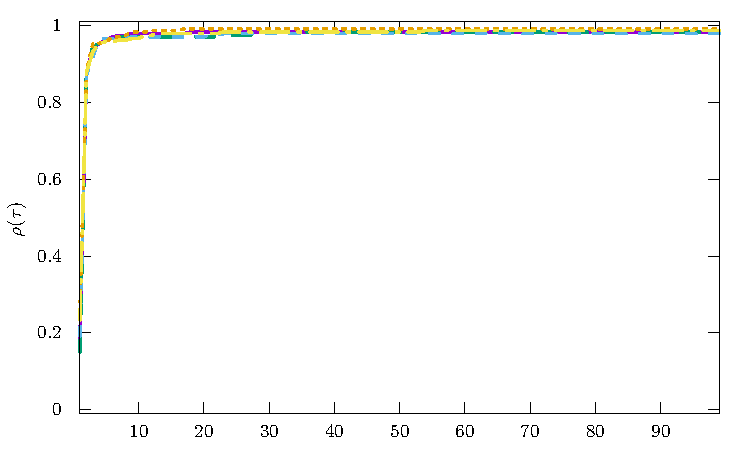
\includegraphics[width=0.7\textwidth]{COMP/large/flpops/profile-Chain.pdf}}
%     \centerline{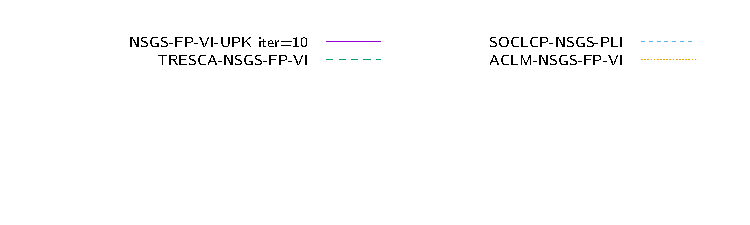
\includegraphics[width=0.7\textwidth]{COMP/large/flpops/profile-Chain_legend.pdf}}
% }

% \subsection{Capsules}

% \frame{
%   \frametitle{First comparisons. Capsules}
%  \begin{block}
%     {100 capsules dropped into a box.}
%     code: Siconos
%     $$ $$
%   \begin{minipage}{0.49\linewidth}
%     \includegraphics[width=1.0\textwidth]{Capsules}
%   \end{minipage}  
%   \begin{minipage}{0.49\linewidth}
%     \begin{tabular}{|p{0.7\textwidth}|c|}
%       coefficient of friction & $0.7$ \\[\ssep]
%       number of problems & 1705 \\[\ssep]
%       number of degrees of freedom & [6 : 600] \\[\ssep]
%       number of contacts &  [0:300]\\[\ssep]
%       required accuracy   & $10^{-8}$    
%     \end{tabular}
%   \end{minipage}
% \end{block}
% }
% \frame{
%   \frametitle{First comparisons. Capsules}
%   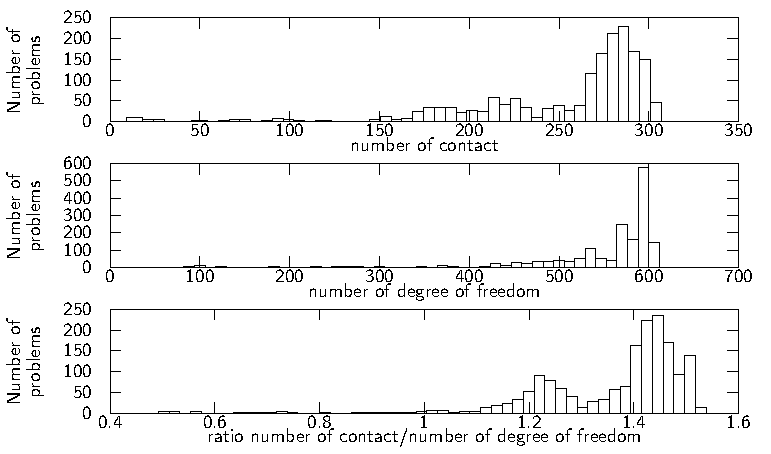
\includegraphics[width=1.10\textwidth]{distrib-Capsules.pdf}
% }
% % \frame{
% %   \frametitle{First comparisons. Capsules}
% %   \centerline{\includegraphics[width=1.10\textwidth]{profile-Capsules.pdf}}
% % }
% \frame{
%   \frametitle{First comparisons. Capsules}
%     \centerline{\includegraphics[width=0.7\textwidth]{COMP/large/flpops/profile-Capsules.pdf}}
%     \centerline{
\includegraphics[width=0.7\textwidth]{COMP/large/flpops/profile-Capsules_legend.pdf}}
% }




% \subsection{Performance profiles. BoxesStack}

% \frame{
%   \frametitle{First comparisons. BoxesStack}
%   \begin{block}
%     {50 boxes stacked under gravity.}
%     code: Siconos
%     $$ $$
%   \begin{minipage}{0.14\linewidth}
%     \includegraphics[width=1.0\textwidth]{BoxesStack}
%   \end{minipage}
%   \begin{minipage}{0.25\linewidth}
%     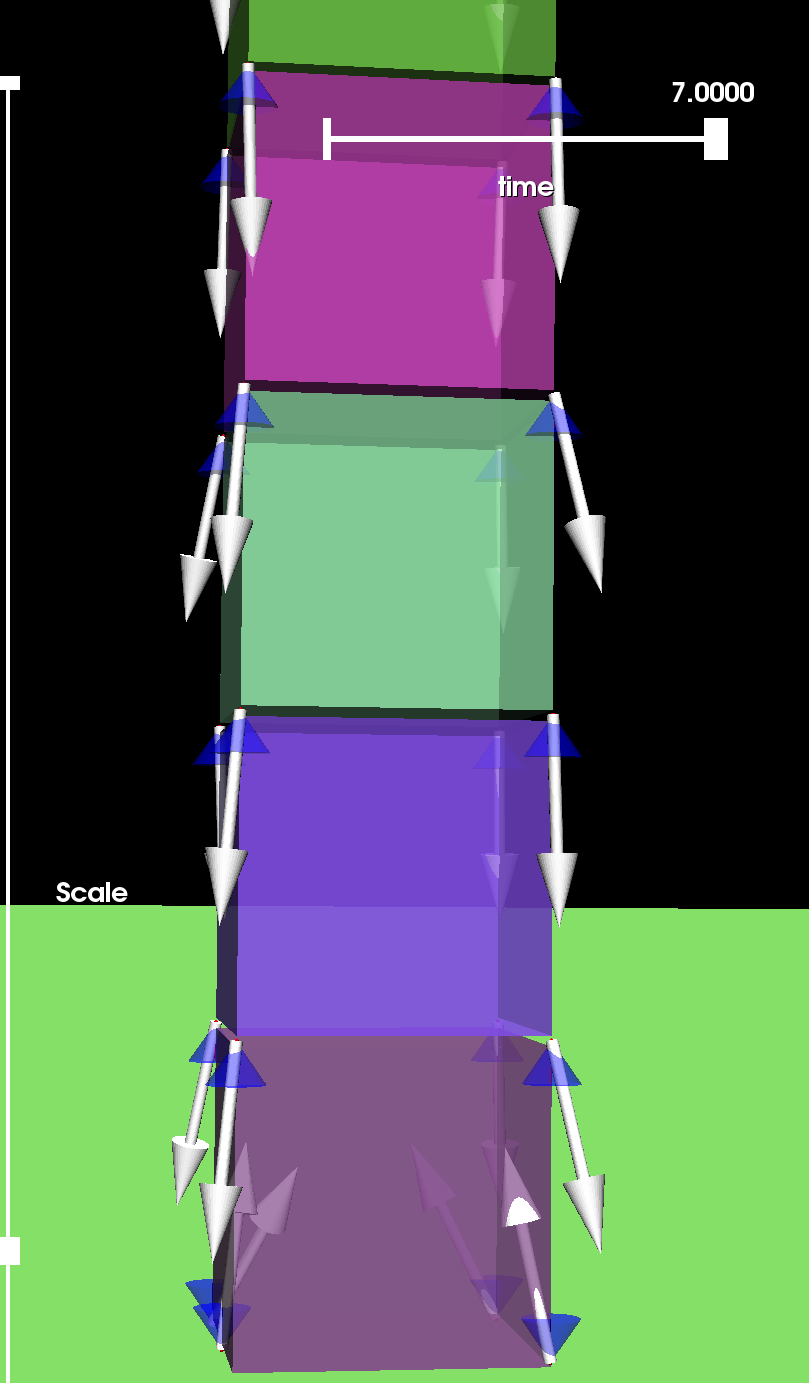
\includegraphics[width=1.0\textwidth]{BoxesStack2}
%   \end{minipage}
%   \begin{minipage}{0.49\linewidth}
%     \begin{tabular}{|p{0.7\textwidth}|c|}
%       coefficient of friction &  0.7\\[\ssep]
%       number of problems &  1159 \\[\ssep]
%       number of degrees of freedom & [6 : 300] \\[\ssep]
%       number of contacts &  [ 0: 200]\\[\ssep]
%       required accuracy   & $10^{-8}$
%     \end{tabular}
%   \end{minipage}
% \end{block}
% }
% \frame{
%   \frametitle{First comparisons. BoxesStack}
%   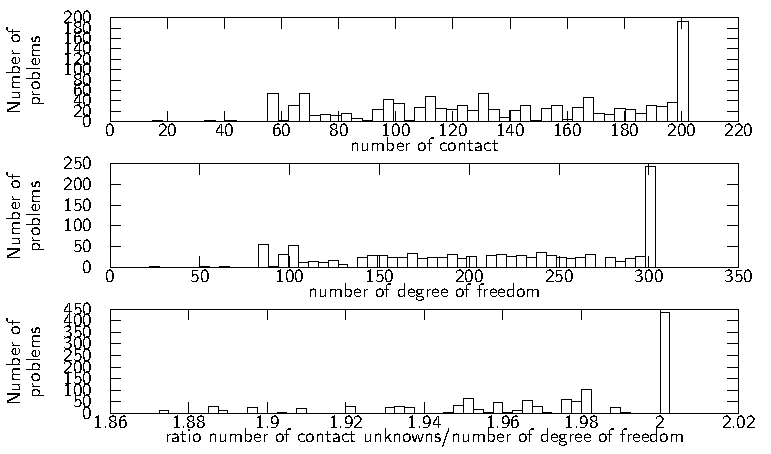
\includegraphics[width=1.10\textwidth]{distrib-BoxesStack1.pdf}
% }
% % \frame{
% %   \frametitle{First comparisons. BoxesStack}
% %   \centerline{\includegraphics[width=1.1\textwidth]{profile-BoxesStack1.pdf}}
% % }
% \frame{
%   \frametitle{First comparisons. BoxesStack1}
%     \centerline{\includegraphics[width=0.7\textwidth]{COMP/large/flpops/profile-BoxesStack1.pdf}}
%     \centerline{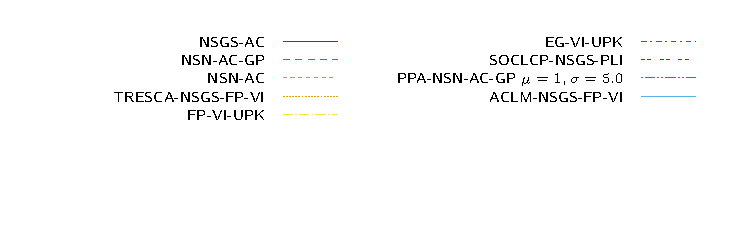
\includegraphics[width=0.7\textwidth]{COMP/large/flpops/profile-BoxesStack1_legend.pdf}}
% }


% \subsection{Performance profiles. Kaplas}

% \frame{
%   \frametitle{A tower of Kaplas}
%   \begin{block}
%     {A Tower of Kaplas}
%     code: Siconos
%     $$ $$
%   \begin{minipage}{0.50\linewidth}
%     \includegraphics[width=1.0\textwidth]{KaplasTower}
%   \end{minipage}
%   \begin{minipage}{0.49\linewidth}
%     \begin{tabular}{|p{0.7\textwidth}|c|}
%       coefficient of friction &  0.3\\[\ssep]
%       number of problems &  201 \\[\ssep]
%       number of degrees of freedom & [72 : 864] \\[\ssep]
%       number of contacts &  [ 0: 950]\\[\ssep]
%       required accuracy   & $10^{-8}$
%     \end{tabular}
%   \end{minipage}
% \end{block}
% }
% \frame{
%   \frametitle{A tower of Kaplas}
%   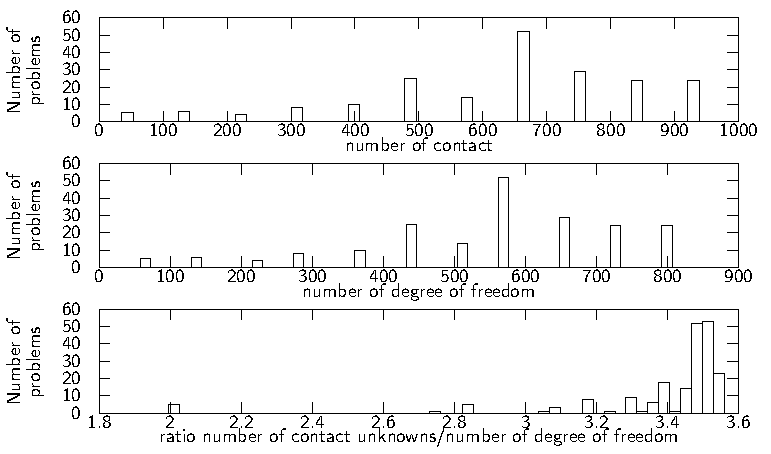
\includegraphics[width=1.10\textwidth]{distrib-KaplasTower.pdf}
% }
% % \frame{
% %   \frametitle{A tower of  Kaplas}
% %   \centerline{\includegraphics[width=1.1\textwidth]{profile-KaplasTower.pdf}}
% % }
% \frame{
%   \frametitle{First comparisons. Kaplas Tower}
%     \centerline{\includegraphics[width=0.7\textwidth]{COMP/large/flpops/profile-KaplasTower.pdf}}
%     \centerline{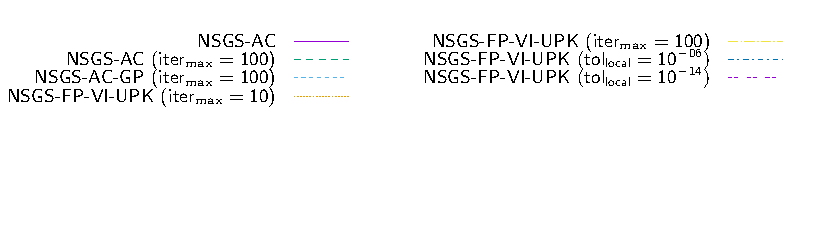
\includegraphics[width=0.7\textwidth]{COMP/large/flpops/profile-KaplasTower_legend.pdf}}
% }
% % \subsection{Performance profiles. AqueducPR}

% % % \frame{An aqueduct}
% % %   \begin{block}
% % %     {An aqueduct}
% % %     code: LMGC
% % %     $$ $$
% % %   \begin{minipage}{0.50\linewidth}
% % %    % \includegraphics[width=1.0\textwidth]{Aqueduc_PR.png}
% % %   \end{minipage}
% % %   \begin{minipage}{0.49\linewidth}
% % %     \begin{tabular}{|p{0.7\textwidth}|c|}
% % %       coefficient of friction &  0.5\\[\ssep]
% % %       number of problems &  10 \\[\ssep]
% % %       number of degrees of freedom & 1932 \\[\ssep]
% % %       number of contacts &  [ 4387: 4477]\\[\ssep]
% % %       required accuracy   & $10^{-4}$
% % %     \end{tabular}
% % %   \end{minipage}
% % % \end{block}
% % % }
% % % \frame{
% % %   \frametitle{An aqueduct}
% % %   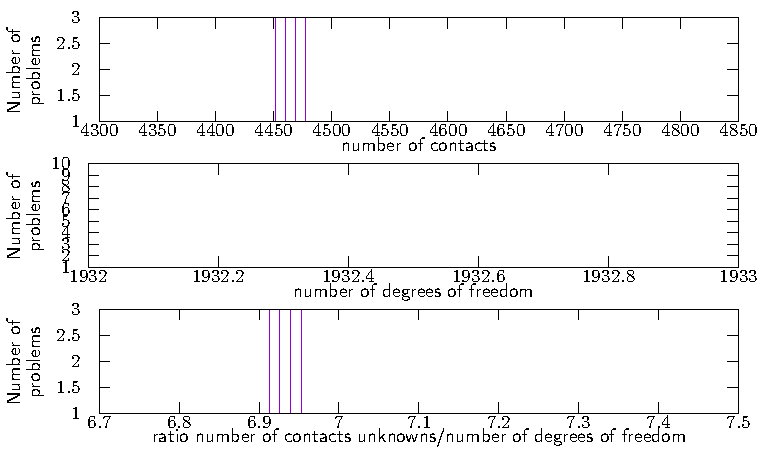
\includegraphics[width=1.10\textwidth]{distrib-LMGC_AqueducPR.pdf}
% % % }
% % % \frame{
% % %   \frametitle{A tower of  Kaplas}
% % %   \centerline{\includegraphics[width=1.1\textwidth]{profile-KaplasTower.pdf}}
% % % }
% % \frame{
% %   \frametitle{First comparisons. An aqueduct}
% %     \centerline{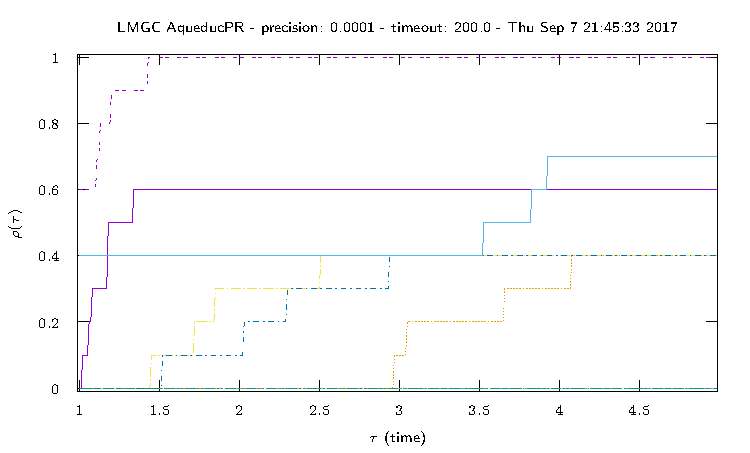
\includegraphics[width=0.7\textwidth]{COMP/large/flpops/profile-LMGC_AqueducPR.pdf}}
% %     \centerline{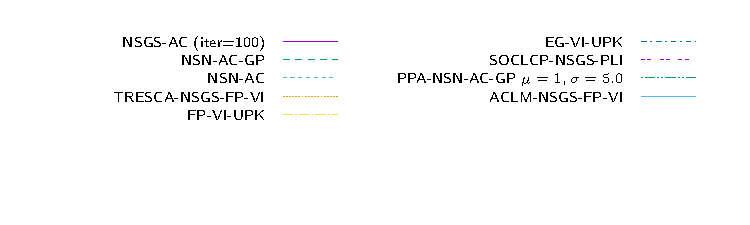
\includegraphics[width=0.7\textwidth]{COMP/large/flpops/profile-LMGC_AqueducPR_legend.pdf}}
% % }





% \subsection{Performance profiles.  FEM Cube H8}

% \frame{
%   \frametitle{Two elastic Cubes with FEM discretization H8}
%   \begin{block}
%     {Two elastic Cubes with FEM discretization H8}
%     code : LMGC90
%     $$ $$
%    \begin{minipage}{0.40\linewidth}
%      \includegraphics[width=1.0\textwidth]{Cubes_H8_5}
%    \end{minipage}
%    \begin{minipage}{0.49\linewidth}
%      \begin{tabular}{|p{0.7\textwidth}|c|}
%        coefficient of friction &  0.3\\[\ssep]
%        number of problems &  58 \\[\ssep]
%        number of degrees of freedom & \{162,1083,55566\} \\[\ssep]
%        number of contacts &  [ 3:5] [30:36]  [360:368 ]\\[\ssep]
%        required accuracy   & $10^{-5}$
%      \end{tabular}
%   \end{minipage}
% \end{block}
% }
% \frame{
%   \frametitle{Two elastic Cubes with FEM discretization H8}
%   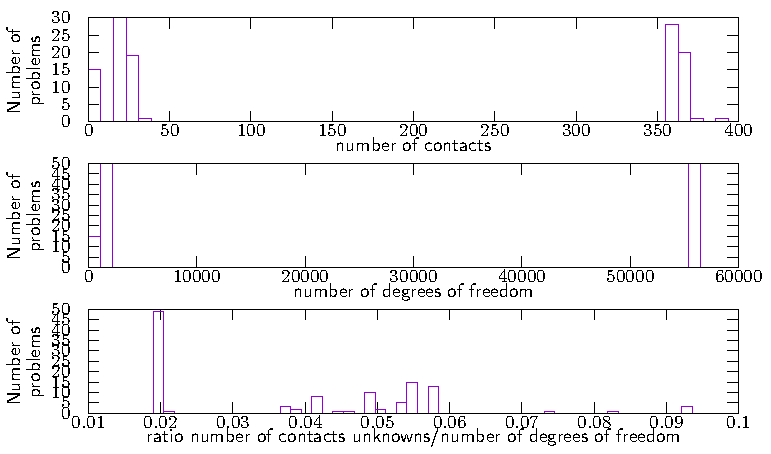
\includegraphics[width=1.10\textwidth]{distrib-LMGC_Cubes_H8_5.pdf}
%  }
% % \frame{
% %   \frametitle{A tower of  Kaplas}
% %   \centerline{\includegraphics[width=1.1\textwidth]{profile-KaplasTower.pdf}}
% % }
% \frame{
%   \frametitle{First comparisons. Cubes H8}
%     \centerline{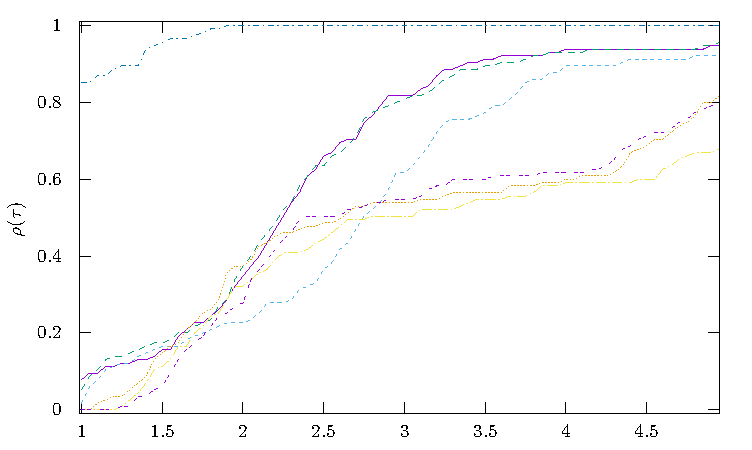
\includegraphics[width=0.7\textwidth]{COMP/large/flpops/profile-LMGC_Cubes_H8.pdf}}
%     \centerline{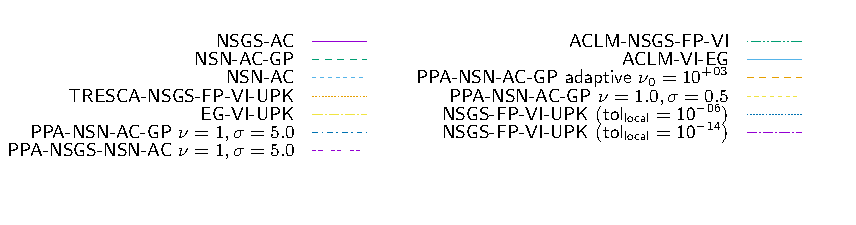
\includegraphics[width=0.7\textwidth]{COMP/large/flpops/profile-LMGC_Cubes_H8_legend.pdf}}
% }

\makeatletter
\def\subfigcounter{\thesubfigure}
%\def\subfigcounter{\thefigure}
\makeatother
\def\subfiglayout{%
  \captionsetup[subfloat]{farskip=-0pt,captionskip=-2pt,font=scriptsize}%
  \setlength{\abovecaptionskip}{0pt}}
%\def\subfiglayout{}
\def\measurename{time}
\def\performance{time}
\def\widthfigure{0.6}
\def\figwidth{0.45\textwidth}
\def\legendwidth{0.6\textwidth}
\def\legendheight{0.20\textheight}
\begin{frame}
  \frametitle{Comparisons by families of solvers}
  \begin{center}
    \begin{figure}
      \centering
      \subfiglayout
      \subfloat[\scriptsize LowWall\_FEM II ($\sf tol =1e^{-04}$)]
      {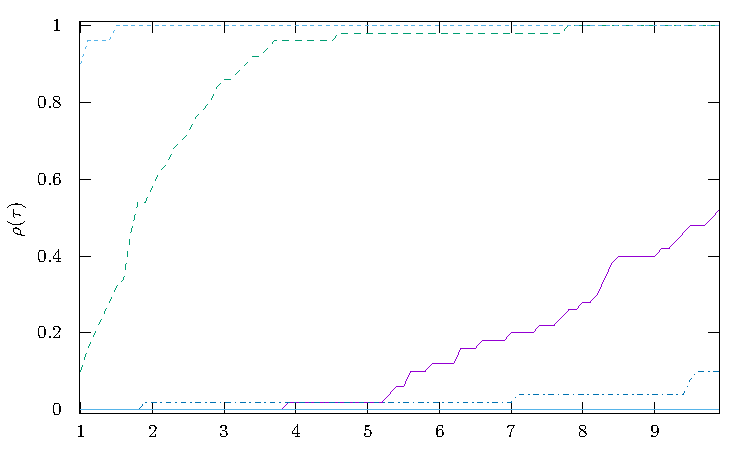
\includegraphics[width=\figwidth]{figure/COMP/large/1.0e-04/400/time/profile-LMGC_LowWall_FEM.pdf}}
      \subfloat[\scriptsize LowWall\_FEM ($\sf tol =1e^{-08}$)]
      {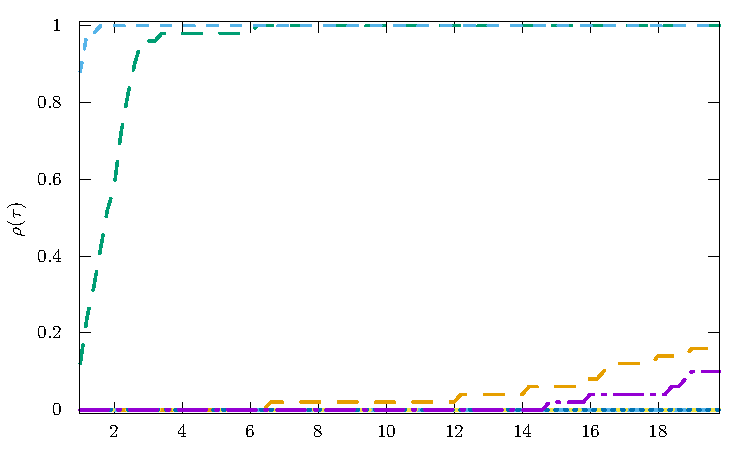
\includegraphics[width=\figwidth]{figure/COMP/large/1.0e-08/400/time/profile-LMGC_LowWall_FEM.pdf}} \\
      % \subfloat[\scriptsize Cubes\_H8 II]
      % {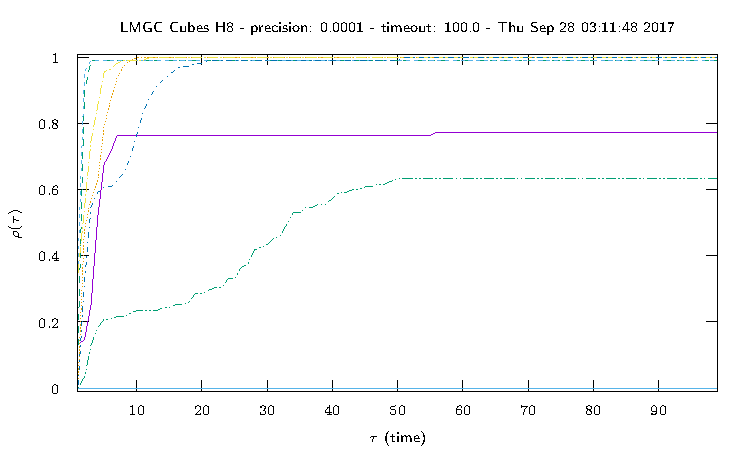
\includegraphics[width=\figwidth]{figure/COMP/large/1.0e-04/100/time/profile-LMGC_Cubes_H8.pdf}} 
      % \subfloat[\scriptsize Cubes\_H8]
      % {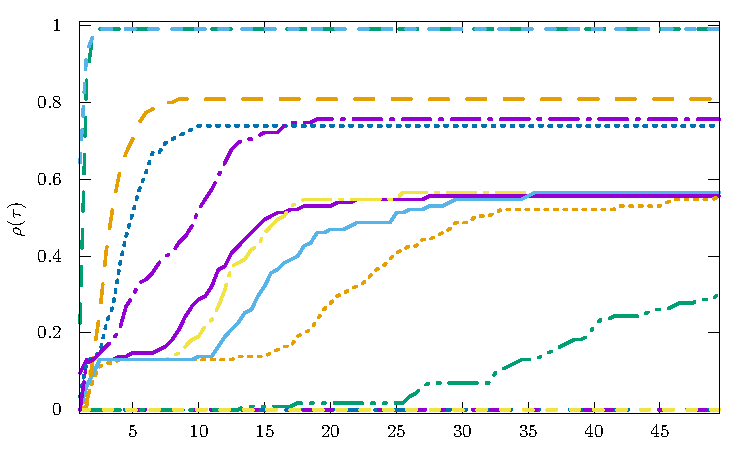
\includegraphics[width=\figwidth]{figure/COMP/large/1.0e-08/100/time/profile-LMGC_Cubes_H8.pdf}} \\
      % \subfloat[\scriptsize Bridge\_PR II]
      % {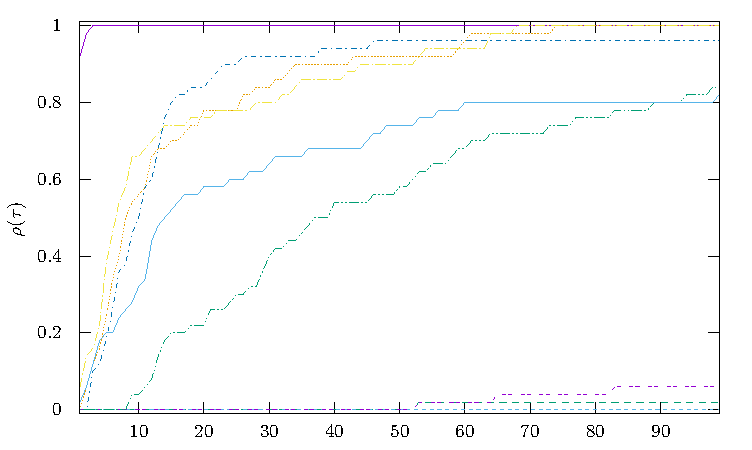
\includegraphics[width=\figwidth]{figure/COMP/large/1.0e-04/100/time/profile-LMGC_Bridge_PR.pdf}} 
      % \subfloat[\scriptsize Bridge\_PR]
      % {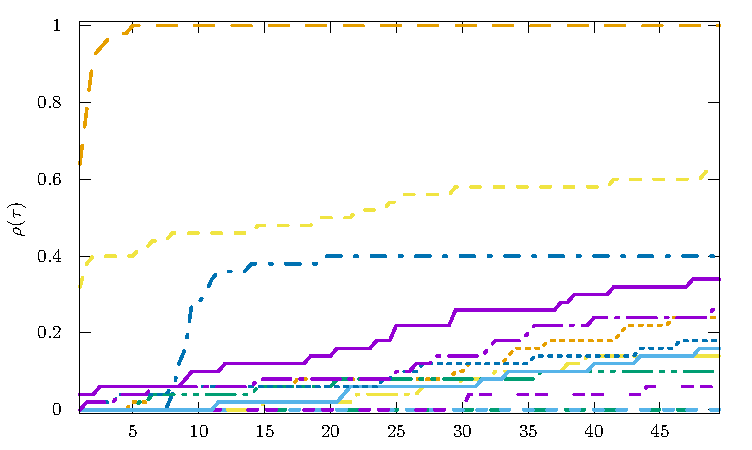
\includegraphics[width=\figwidth]{figure/COMP/large/1.0e-08/400/time/profile-LMGC_Bridge_PR.pdf}} \\
      % \subfloat[\scriptsize AqueducPR]
      % {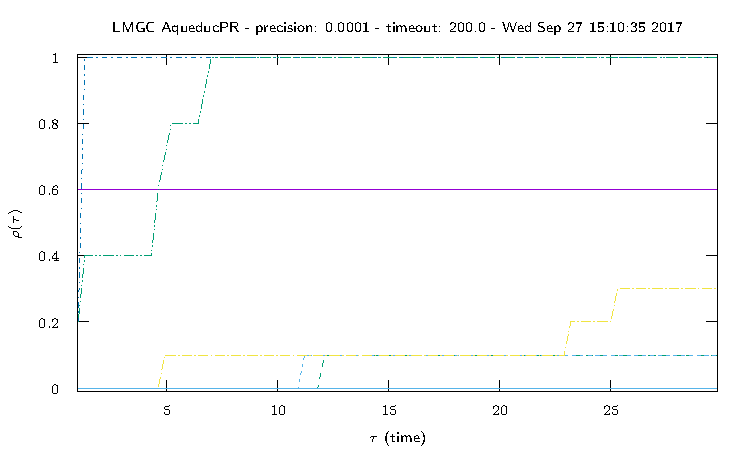
\includegraphics[width=\figwidth]{figure/COMP/large/1.0e-04/200/time/profile-LMGC_AqueducPR.pdf}} 
      \subfloat[\scriptsize 945\_SP\_Box\_PL]
      {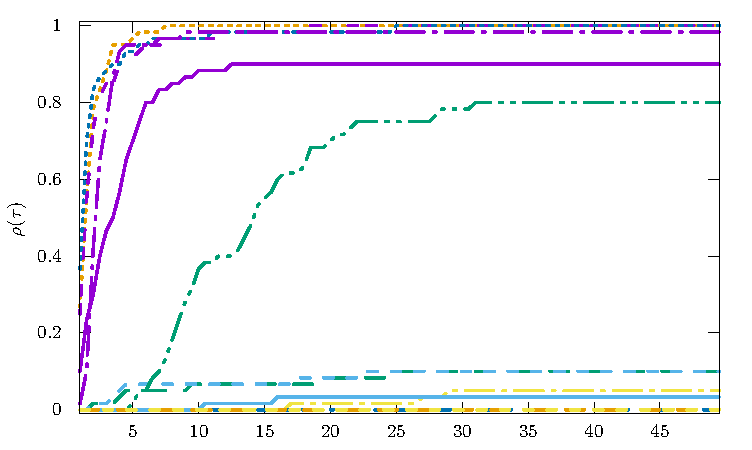
\includegraphics[width=\figwidth]{figure/COMP/large/1.0e-04/100/time/profile-LMGC_945_SP_Box_PL.pdf}} 
      \subfloat[\scriptsize 100\_PR\_PerioBox]
      {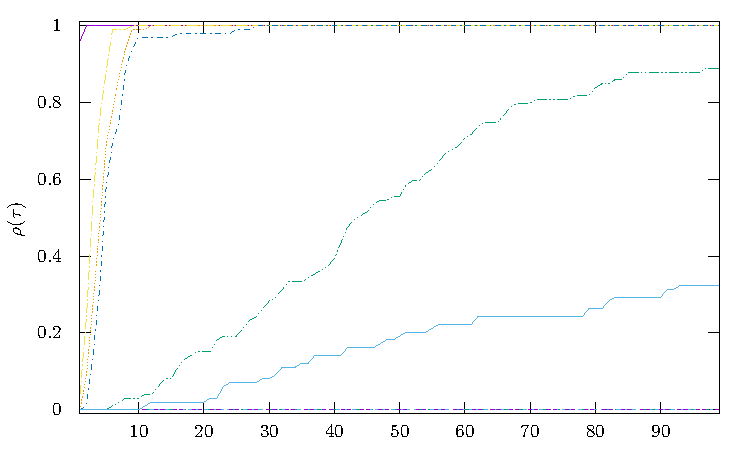
\includegraphics[width=\figwidth]{figure/COMP/large/1.0e-04/100/time/profile-LMGC_100_PR_PerioBox.pdf}}\\
      \includegraphics[height=\legendheight]{figure/COMP/large/1.0e-08/50/time/profile-Chain_legend.pdf}
      %\caption{Comparison of the solvers between families}
    \end{figure}
  
\end{center}
\end{frame}

%%% Local Variables:
%%% mode: latex
%%% TeX-master: "s"
%%% End:

